%% NEW VERSION
% marek Thu Nov 29 12:16:01 PST 2012
%          still a lot of work needed. 
% marek Tue Dec  4 12:54:24 PST 2012
% marek Mon Dec 10 18:48:31 PST 2012
% marek Tue Feb 26 17:58:29 PST 2013
% marek Thu Feb 28 15:15:30 PST 2013


\section{Algorithm~{\EBGS} with Ratio $1.575$}\label{sec: 1.575-approximation}

In this section we give our main result, a $1.575$-approximation
algorithm for $\FTFP$, where $1.575$ is the value of $\min_{\gamma\geq
  1}\max\{\gamma, 1+2/e^\gamma, \frac{1/e+1/e^\gamma}{1-1/\gamma}\}$,
rounded to three decimal digits. This matches the ratio of the best
known LP-rounding algorithm for UFL by
Byrka~{\etal}~\cite{ByrkaGS10}. 

Recall that in Section~\ref{sec: 1.736-approximation} we showed how to
compute an integral solution with facility cost bounded by $F^\ast$
and connection cost bounded by $C^\ast + 2/e\cdot\LP^\ast$. Thus, while our
facility cost does not exceed the optimal fractional facility cost, our connection
cost is significantly larger than the connection cost in the optimal fractional solution.
A natural idea is to balance these two ratios by reducing the connection cost at the
expense of the facility cost. One way to do
this would be to increase the probability of opening facilities, from
$\bary_{\mu}$ (used in Algorithm~{\ECHS}) to, say,
$\gamma\bary_{\mu}$, for some $\gamma > 1$. This increases the
expected facility cost by a factor of $\gamma$ but, as it turns out,
it also reduces the probability that an indirect connection occurs for
a non-primary demand to $1/e^\gamma$ (from the previous value
$1/e$). Moreover, for each primary demand $\kappa$, the new algorithm
will select a facility from the nearest facilities $\mu$ in
$\wbarN(\kappa)$ such that the connection values $\barx_{\mu\nu}$
sum up to $1/\gamma$, instead of $1$. It is easily seen that this will
improve the estimate on connection cost for primary demands.  These
two changes, along with a more refined analysis, are the essence of
the approach in~\cite{ByrkaGS10}, expressed in our terminology.

Our approach can be thought of as a combination of the above ideas
with the techniques of demand reduction and
adaptive partitioning that we introduced earlier. However, our
adaptive partitioning technique needs to be carefully modified,
because now we will be using a more intricate neighborhood structure,
with the neighborhood of each demand divided into two disjoint parts,
and with some restrictions on how parts from different demands can overlap.

We begin by describing properties that our partitioned fractional
solution $(\barbfx,\barbfy)$ needs to satisfy. Assume that $\gamma$ is
some constant such that $1 < \gamma < 2$. As mentioned earlier,
the neighborhood $\wbarN(\nu)$ of each demand $\nu$ will be divided
into two disjoint parts.  The first part, called the \emph{close
  neighborhood} and denoted $\wbarclsnb(\nu)$, contains the facilities
in $\wbarN(\nu)$ nearest to $\nu$ with the total connection value
equal $1/\gamma$, that is $\sum_{\mu\in\wbarclsnb(\nu)} \barx_{\mu\nu}
= 1/\gamma$.  The second part, called the \emph{far neighborhood} and
denoted $\wbarfarnb(\nu)$, contains the remaining facilities in
$\wbarN(\nu)$ (so $\sum_{\mu\in\wbarfarnb(\nu)} \barx_{\mu\nu} = 1-1/\gamma$).  We
restate these definitions formally below in Property~(NB).  Recall
that for any set $A$ of facilities and a demand $\nu$, by
$D(A,\nu)$ we denote the average distance between $\nu$ and the
facilities in $A$, that is $D(A,\nu) =\sum_{\mu\in A}
d_{\mu\nu}\bary_{\mu}/\sum_{\mu\in A} \bary_{\mu}$.  We will use
notations $\clsdist(\nu)=D(\wbarclsnb(\nu),\nu)$ and
$\fardist(\nu)=D(\wbarfarnb(\nu),\nu)$ for the average distances from
$\nu$ to its close and far neighborhoods, respectively.  By the
definition of these sets and the completeness property (CO), these
distances can be expressed as
%
\begin{equation*}
\clsdist(\nu)=\gamma\sum_{\mu\in\wbarclsnb(\nu)}
			d_{\mu\nu}\barx_{\mu\nu} \quad\text{and}\quad
\fardist(\nu)=\frac{\gamma}{\gamma-1}\sum_{\mu\in\wbarfarnb(\nu)}
d_{\mu\nu}\barx_{\mu\nu}. 
\end{equation*}
%
We will also use
notation $\clsmax(\nu)=\max_{\mu\in\wbarclsnb(\nu)} d_{\mu\nu}$ for
the maximum distance from $\nu$ to its close neighborhood.

Our partitioned solution $(\barbfx,\barbfy)$ must satisfy the same
partitioning and completeness properties as before, namely properties
(PS) and (CO) in Section~\ref{sec: adaptive partitioning}.  In
addition, it must satisfy a new neighborhood property (NB) and modified
properties (PD') and (SI'), listed below.

\begin{description}
	
      \renewcommand{\theenumii}{(\alph{enumii})}
      \renewcommand{\labelenumii}{\theenumii}

\item{(NB)} \label{NB}
	\emph{Neighborhoods.}
	For each demand $\nu \in \demandset$, its neighborhood is divided into \emph{close} and
	\emph{far} neighborhood, that is $\wbarN(\nu) = \wbarclsnb(\nu) \cup \wbarfarnb(\nu)$, where
	%
	\begin{itemize}
	\item $\wbarclsnb(\nu) \cap \wbarfarnb(\nu) = \emptyset$,
	\item $\sum_{\mu\in\wbarclsnb(\nu)} \barx_{\mu\nu} =1/\gamma$, and 
	\item if $\mu\in \wbarclsnb(\nu)$ and $\mu'\in \wbarfarnb(\nu)$ 
				then $d_{\mu\nu}\le d_{\mu'\nu}$.   
	\end{itemize}
	%
	Note that the first two conditions, together with
        (PS.\ref{PS:one}), imply that $\sum_{\mu\in\wbarfarnb(\nu)}
        \barx_{\mu\nu} =1-1/\gamma$.

\item{(PD')} \emph{Primary demands.}
	Primary demands satisfy the following conditions:

	\begin{enumerate}
		
	\item\label{PD1:disjoint}  For any two different primary demands $\kappa,\kappa'\in P$ we have
				$\wbarclsnb(\kappa)\cap \wbarclsnb(\kappa') = \emptyset$.

	\item \label{PD1:yi} For each site $i\in\sitesset$, 
		$ \sum_{\kappa\in P}\sum_{\mu\in
                  i\cap\wbarclsnb(\kappa)}\barx_{\mu\kappa} \leq
                y_i^\ast$. In the summation, as before, we overload notation $i$ to stand for the set of
						facilities created on site $i$.
		
	\item \label{PD1:assign} Each demand $\nu\in\demandset$ is assigned
        to one primary demand $\kappa\in P$ such that

  			\begin{enumerate}
	
				\item \label{PD1:assign:overlap} $\wbarclsnb(\nu) \cap \wbarclsnb(\kappa) \neq \emptyset$, and
				%
				\item \label{PD1:assign:cost}
          $\clsdist(\nu)+\clsmax(\nu) \geq
          \clsdist(\kappa)+\clsmax(\kappa)$.
          %
			\end{enumerate}

	\end{enumerate}
	
\item{(SI')} \emph{Siblings}. For any pair $\nu,\nu'\in\demandset$ of different siblings we have
  \begin{enumerate}

	\item \label{SI1:siblings disjoint}
		  $\wbarN(\nu)\cap \wbarN(\nu') = \emptyset$.
		
	\item \label{SI1:primary disjoint} If $\nu$ is assigned to a primary demand $\kappa$ then
 		$\wbarN(\nu')\cap \wbarclsnb(\kappa) = \emptyset$. In particular, by Property~(PD'.\ref{PD1:assign:overlap}),
		this implies that different sibling demands are assigned to different primary demands, since $\wbarclsnb(\nu')$ is a subset of $\wbarN(\nu')$.

	\end{enumerate}
	
\end{description}

%%%%%%%%%%%%%%%%%

\paragraph{Modified adaptive partitioning.}
To obtain a fractional solution with the above properties, we employ a
modified adaptive partitioning algorithm. As in Section~\ref{sec:
  adaptive partitioning}, we have two phases.  In Phase~1 we split
clients into demands and create facilities on sites, while in Phase~2
we augment each demand's connection values $\barx_{\mu\nu}$ so that the total connection
value of each demand $\nu$ is $1$. As the partitioning algorithm proceeds, for any demand $\nu$,
$\wbarN(\nu)$ denotes the set of facilities with $\barx_{\mu\nu} > 0$;
hence the notation $\wbarN(\nu)$ actually represents a dynamic set which gets fixed 
once the partitioning algorithm concludes both Phase 2. On the
other hand, $\wbarclsnb(\nu)$ and $\wbarfarnb(\nu)$ refer to the close
and far neighborhoods at the time when $\wbarN(\nu)$ is fixed.

Similar to the algorithm in Section~\ref{sec: adaptive partitioning},
Phase~1 runs in iterations. Fix some iteration and consider any client
$j$.  As before, $\wtildeN(j)$ is the neighborhood of $j$ with respect
to the yet unpartitioned solution, namely the set of facilities $\mu$
such that $\tildex_{\mu j}>0$. Order the facilities in this set as
$\wtildeN(j) = \braced{\mu_1,...,\mu_q}$ with non-decreasing distance
from $j$, that is $d_{\mu_1 j} \leq d_{\mu_2 j} \leq \ldots \leq
d_{\mu_q j}$. Without loss of generality,
there is an index $l$ for which $\sum_{s=1}^l \tildex_{\mu_s j} =
1/\gamma$, since we can always split one facility to achieve
this. Then we define $\wtildeclsnb(j) = \braced{\mu_1,...,\mu_l}$. 
(Unlike close neighborhoods of demands, $\wtildeclsnb(j)$ can vary over time.)
In case of ties, which can occur when some facilities in $\wtildeN(j)$ are at the same
distance from $j$, we use a tie-breaking rule that is explained in the
proof of Lemma~\ref{lem: PD1: primary overlap} (the only place where
the rule is needed). We also use notation
%
\begin{equation*}
\tcccls(j) =  D(\wtildeclsnb(j), j) = \gamma\sum_{\mu\in\wtildeclsnb(j)} d_{\mu j} \tildex_{\mu j}
			\quad\textrm{ and }\quad
 \dmaxcls(j) = \max_{\mu \in \wtildeclsnb(j)} d_{\mu j}. 
\end{equation*}
%

When the iteration starts, we first find a not-yet-exhausted client
$p$ that minimizes the value of $\tcccls(p) + \dmaxcls(p)$ and create
a new demand $\nu$ for $p$.  Now we have two cases:
%
\begin{description}
%
\item{\mycase{1}} $\wtildeclsnb(p) \cap \wbarN(\kappa)\neq\emptyset$
  for some existing primary demand $\kappa\in P$.  In this case we
  assign $\nu$ to $\kappa$. As before, if there are multiple such
  $\kappa$, we pick any of them. We also fix $\barx_{\mu \nu} \assign
  \tildex_{\mu p}$ and $\tildex_{\mu p}\assign 0$ for each $\mu \in
  \wtildeN(p)\cap \wbarN(\kappa)$. Note that although we
  check for overlap between $\wtildeclsnb(p)$ and $\wbarN(\kappa)$,
  the facilities we actually move into $\wbarN(\nu)$ include all
  facilities in the intersection of $\wtildeN(p)$, a bigger set, with
  $\wbarN(\kappa)$.

  At this time, the total connection value 
	between $\nu$ and $\mu\in \wbarN(\nu)$ is at most $1/\gamma$,
	 since $\sum_{\mu \in \wbarN(\kappa)}\bary_{\mu} = 1/\gamma$ 
	(this follows from the definition of neighborhoods for new primary demands in Case~2 below) 
	and  we have $\wbarN(\nu) \subseteq \wbarN(\kappa)$ at this point. Later
  in Phase 2 we will add additional facilities from $\wtildeN(p)$ to
  $\wbarN(\nu)$ to make $\nu$'s total connection value equal to $1$.

%
\item{\mycase{2}} $\wtildeclsnb(p) \cap \wbarN(\kappa) = \emptyset$
  for all existing primary demands $\kappa\in P$.  In this case we
  make $\nu$ a primary demand (that is, add it to $P$) and assign it
  to itself.  We then move the facilities from $\wtildeclsnb(p)$ to
  $\wbarN(\nu)$, that is for $\mu \in \wtildeclsnb(p)$ we set
  $\barx_{\mu \nu}\assign \tildex_{\mu p}$ and $\tildex_{\mu p}\set
  0$.

  It is easy to see that the total connection value of $\nu$ to
  $\wbarN(\nu)$ is now exactly $1/\gamma$, that is
	$\sum_{\mu \in \wbarN(\nu)}\bary_{\mu} = 1/\gamma$.
Moreover, facilities
  remaining in $\wtildeN(p)$ are all farther away from $\nu$ than
  those in $\wbarN(\nu)$. As we add only facilities from $\wtildeN(p)$
  to $\wbarN(\nu)$ in Phase~2, the final $\wbarclsnb(\nu)$ contains
  the same set of facilities as the current set $\wbarN(\nu)$.
  (More precisely, $\wbarclsnb(\nu)$ consists of the facilities that
	either are currently in $\wbarN(\nu)$ or were obtained from splitting
	the facilities currently in $\wbarN(\nu)$.)
%
\end{description}
%
Once all clients are exhausted, that is, each client $j$ has $r_j$
demands created, Phase~1 concludes. We then run Phase~2, the
augmenting phase, following the same steps as in Section~\ref{sec:
  adaptive partitioning}.  For each client $j$ and each demand $\nu\in
j$ with total connection value to $\wbarN(\nu)$ less than $1$
(that is, $\sum_{\mu\in\wbarN(\nu)} \barx_{\mu\nu} < 1$),
we use our $\AugmentToUnit()$
procedure to add additional facilities (possibly split, if necessary)
from $\wtildeN(j)$ to $\wbarN(\nu)$ to make the total connection value
between $\nu$ and $\wbarN(\nu)$ equal $1$.

\medskip

This completes the description of the partitioning
algorithm. Summarizing, for each client $j\in\clientset$ we 
created $r_j$ demands on the same point as $j$, and we created a number
of facilities at each site $i\in\sitesset$. Thus computed sets of
demands and facilities are denoted $\demandset$ and $\facilityset$,
respectively.  For each facility $\mu\in i$ we defined its fractional
opening value $\bary_\mu$, $0\le \bary_\mu\le 1$, and for each demand
$\nu\in j$ we defined its fractional connection value
$\barx_{\mu\nu}\in \braced{0,\bary_\mu}$.  The connections with
$\barx_{\mu\nu} > 0$ define the neighborhood $\wbarN(\nu)$. The facilities in
$\wbarN(\nu)$ that are closest to $\nu$ and have total connection value from $\nu$ equal
$1/\gamma$ form the close neighborhood $\wbarclsnb(\nu)$, while the remaining facilities
in $\wbarN(\nu)$ form the far neighborhood
$\wbarfarnb(\nu)$. It remains to show that this partitioning satisfies all the desired
properties.

%%%%%%%

\medskip
\paragraph{Correctness of partitioning.}
We now argue that our partitioned fractional solution $(\barbfx,\barbfy)$
satisfies all the stated properties. Properties~(PS), (CO) and (NB) are
directly enforced by the algorithm.

(PD'.\ref{PD1:disjoint}) holds because for each primary demand
$\kappa\in p$, $\wbarclsnb(\kappa)$ is the same set as
$\wtildeclsnb(p)$ at the time when $\kappa$ was created, and
$\wtildeclsnb(p)$ is removed from $\wtildeN(p)$ right after this
step. Further, the partitioning algorithm makes $\kappa$ a primary
demand only if $\wtildeclsnb(p)$ is disjoint from the set
$\wbarN(\kappa')$ of all existing primary demands $\kappa'$ at that
iteration, but these neighborhoods are the same as the final close
neighborhoods $\wbarclsnb(\kappa')$.

The justification of (PD'.\ref{PD1:yi}) is similar to that for
(PD.\ref{PD:yi}) from Section~\ref{sec: adaptive partitioning}. All
close neighborhoods of primary demands are disjoint, due to
(PD'.\ref{PD1:disjoint}), so each facility $\mu \in i$ can appear in
at most one $\wbarclsnb(\kappa)$, for some $\kappa\in P$. Condition
(CO) implies that $\bary_{\mu} = \barx_{\mu\kappa}$ for $\mu \in \wbarclsnb(\kappa)$.
As a result, the summation on
the left-hand side is not larger than $\sum_{\mu\in i}\bary_{\mu} = y_i^\ast$.

Regarding (PD'.\ref{PD1:assign:overlap}), at first glance this
property seems to follow directly from the algorithm, as we only
assign a demand $\nu$ to a primary demand $\kappa$ when $\wbarN(\nu)$
at that iteration overlaps with $\wbarN(\kappa)$ (which is equal to
the final value of $\wbarclsnb(\kappa)$).  However, it is a little
more subtle, as the final $\wbarclsnb(\nu)$ may contain facilities
added to $\wbarN(\nu)$ in Phase 2. Those facilities may turn out to be
closer to $\nu$ than some facilities in $\wbarN(\kappa) \cap
\wtildeN(j) $ (not $\wtildeN_{\cls}(j)$) that we added to
$\wbarN(\nu)$ in Phase 1. If the final $\wbarclsnb(\nu)$ consists only of
facilities added in Phase 2, we no longer have the desired overlap of
$\wbarclsnb(\kappa)$ and $\wbarclsnb(\nu)$. Luckily this bad scenario
never occurs. We postpone the proof of this property to
Lemma~\ref{lem: PD1: primary overlap}.  The proof of
(PD'.\ref{PD1:assign:cost}) is similar to that of Lemma~\ref{lem:
  PD:assign:cost holds}, and we defer it to Lemma~\ref{lem: PD1:
  primary optimal}.

(SI'.\ref{SI1:siblings disjoint}) follows directly from the algorithm
because for each demand $\nu\in j$, all facilities added to
$\wbarN(\nu)$ are immediately removed from $\wtildeN(j)$ and each
facility is added to $\wbarN(\nu)$ of exactly one demand $\nu \in j$.
Splitting facilities obviously preserves (SI'.\ref{SI1:siblings disjoint}).

The proof of (SI'.\ref{SI1:primary disjoint}) is similar to that of
Lemma~\ref{lem: property SI:primary disjoint holds}. If $\kappa=\nu$
then (SI'.\ref{SI1:primary disjoint}) follows from
(SI'.\ref{SI1:siblings disjoint}), so we can assume that
$\kappa\neq\nu$.  Suppose that $\nu'\in j$ is assigned to $\kappa'\in
P$ and consider the situation after Phase~1. By the way we reassign
facilities in Case~1, at this time we have $\wbarN(\nu)\subseteq
\wbarN(\kappa) = \wbarclsnb(\kappa)$ and $\wbarN(\nu')\subseteq
\wbarN(\kappa') =\wbarclsnb(\kappa')$, so $\wbarN(\nu')\cap
\wbarclsnb(\kappa) = \emptyset$, by (PD'.\ref{PD1:disjoint}).
Moreover, we have $\wtildeN(j) \cap \wbarclsnb(\kappa) = \emptyset$
after this iteration, because any facilities that were also in
$\wbarclsnb(\kappa)$ were removed from $\wtildeN(j)$ when $\nu$ was
created. In Phase~2, augmentation does not change $\wbarclsnb(\kappa)$
and all facilities added to $\wbarN(\nu')$ are from the set
$\wtildeN(j)$ at the end of Phase 1, which is a subset of the set
$\wtildeN(j)$ after this iteration, since $\wtildeN(j)$ can only shrink. 
So the condition (SI'.\ref{SI1:primary disjoint}) will
remain true.

%%%%%%%%%%%%%%%

\begin{lemma} \label{lem: PD1: primary overlap}
  Property (PD'.\ref{PD1:assign:overlap}) holds.
\end{lemma}

\begin{proof}
  Let $j$ be the client for which $\nu\in j$. We consider an iteration
  when we create $\nu$ from $j$ and assign it to $\kappa$, and
  within this proof, notation $\wtildeclsnb(j)$ and $\wtildeN(j)$
  will refer to the value of the sets at this particular time.  
% if reviewers complain, we can introduce superscript v to indicate that
% as we do elsewhere
At this time, $\wbarN(\nu)$ is initialized to $\wtildeN(j)\cap
  \wbarN(\kappa)$.  Recall that $\wbarN(\kappa)$ is now equal to the
  final $\wbarclsnb(\kappa)$ (taking into account facility splitting). We
  would like to show that the set $\wtildeclsnb(j)\cap
  \wbarclsnb(\kappa)$ (which is not empty) will be included in
  $\wbarclsnb(\nu)$ at the end. Technically speaking, this will not be
  true due to facility splitting, so we need to rephrase this claim
  and the proof in terms of the set of facilities obtained after the
  algorithm completes.

\begin{figure}[ht]
\begin{center}
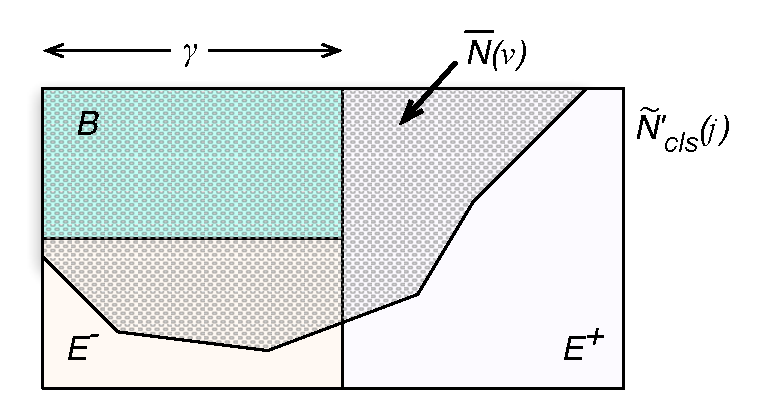
\includegraphics[width=3.2in]{./FIGURES/proof_of_lemma_PD'3a.pdf}
\caption{Illustration of the sets $\wbarN(\nu)$, $A$, $B$,
  $E^-$ and $E^+$ in the proof of Lemma~\ref{lem: PD1:
    primary overlap}. Let $X \Subset Y$ mean that the facility
	sets $X$ is obtained from $Y$ by splitting facilities.
	We then have $A \Subset \wtildeN(j)$, 
	$B \Subset  \wtildeclsnb(j) \cap \wbarclsnb(\kappa)$, 
	$E^- \Subset  \wtildeclsnb(j) - \wbarclsnb(\kappa)$, 
	$E^+ \Subset \wtildeN(j) - \wtildeclsnb(j)$.}
\label{fig: sets lemma PD'3a}
\end{center}
\end{figure}

  We define the sets $A$, $B$, $E^-$ and $E^+$ as the subsets of
  $\facilityset$ (the final set of facilities) that were obtained from
  splitting facilities in the sets $\wtildeN(j)$, $\wtildeclsnb(j)\cap
  \wbarclsnb(\kappa)$, $\wtildeclsnb(j) - \wbarclsnb(\kappa)$ and
  $\wtildeN(j) - \wtildeclsnb(j)$, respectively.  (See
  Figure~\ref{fig: sets lemma PD'3a}.)  We claim that at the end
  $B\subseteq \wbarclsnb(\nu)$, with the caveat that the ties in the
  definition of $\wbarclsnb(\nu)$ are broken in favor of the
  facilities in $B$.  (This is the tie-breaking rule that we mentioned
  in the definition of $\wbarclsnb(\nu)$.)  This will be sufficient to
  prove the lemma because $B\neq\emptyset$, by the algorithm.

  We now prove this claim. In this paragraph $\wbarN(\nu)$ denotes the
  final set $\wbarN(\nu)$ after both phases are completed. Thus the total
connection value of $\wbarN(\nu)$ to $\nu$ is $1$.
	Note first that
  $B\subseteq \wbarN(\nu) \subseteq A$, because we never remove
  facilities from $\wbarN(\nu)$ and we only add facilities from
  $\wtildeN(j)$.  Also, $B\cup E^-$ represents the facilities obtained
  from $\wtildeclsnb(j)$, so $\sum_{\mu\in B\cup E^-} \bary_{\mu} =
  1/\gamma$.  This and $B\subseteq \wbarN(\nu)$ implies that the total
  connection value of $B\cup (\wbarN(\nu)\cap E^-)$ to $\nu$ is at
  most $1/\gamma$. But all facilities in $B\cup (\wbarN(\nu)\cap E^-)$
  are closer to $\nu$ (taking into account our tie breaking)
 	than those in $E^+\cap \wbarN(\nu)$. It follows
  that $B\subseteq \wbarclsnb(\nu)$, completing the proof.
\end{proof}

%%%%%%%%%%%%%%

\begin{lemma}\label{lem: PD1: primary optimal}
  Property (PD'.\ref{PD:assign:cost}) holds.
\end{lemma}

\begin{proof}
This proof is similar to that for Lemma~\ref{lem: PD:assign:cost holds}.
For a client $j$ and demand $\eta$, we will write
$\tcccls^\eta(j)$ and $\dmaxcls^\eta(j)$ to denote the values of
$\tcccls(j)$ and $\dmaxcls(j)$ at the time when $\eta$
was created. (Here $\eta$ may or may not be a demand of client $j$).

Suppose $\nu \in j$ is assigned to a primary demand $\kappa \in p$.
By the way primary demands are constructed in the partitioning
algorithm, $\wtildeclsnb(p)$ becomes $\wbarN(\kappa)$, which is equal
to the final value of $\wbarclsnb(\kappa)$. So we have
$\clsdist(\kappa) = \tcccls^\kappa (p)$ and $\clsmax(\kappa) =
\dmaxcls^\kappa(p)$. Further, since we choose $p$ to minimize
$\tcccls(p) + \dmaxcls(p)$, we have that $\tcccls^\kappa(p) +
\dmaxcls^\kappa(p) \leq \tcccls^\kappa(j) + \dmaxcls^\kappa(j)$.

Using an argument analogous to that in the proof of Lemma~\ref{lem: tcc optimal}, 
our modified partitioning algorithm guarantees that
  $\tcccls^{\kappa}(j) \leq \tcccls^{\nu}(j) \leq \clsdist(\nu)$ and
  $\dmaxcls^{\kappa}(j) \leq \dmaxcls^{\nu}(j) \leq \clsmax(\nu)$ since $\nu$ was
  created later.
  Therefore, we have
%
%\margincomment{the last equality seems false}
  \begin{align*}
    \clsdist(\kappa) + \clsmax(\kappa) &= \tcccls^{\kappa}(p) +	\dmaxcls^{\kappa}(p) 
					\\
					&\leq \tcccls^{\kappa}(j) + \dmaxcls^{\kappa}(j) 
					\leq \tcccls^{\nu}(j) + \dmaxcls^{\nu}(j) 
					\leq \clsdist(\nu) + \clsmax(\nu),
  \end{align*}
%
completing the proof.
\end{proof}

%%%%%%%%

Now we have completed the proof that the computed partitioning satisfies
all the required properties. 


\paragraph{Algorithm~{\EBGS}.}
The complete algorithm starts with solving the LP(\ref{eqn:fac_primal}) and
computing the partitioning described earlier in this section.  Given
the partitioned fractional solution $(\barbfx, \barbfy)$ with the
desired properties, we start the process of opening facilities and
making connections to obtain an integral solution. To this end, for
each primary demand $\kappa\in P$, we open exactly one facility
$\phi(\kappa)$ in $\wbarclsnb(\kappa)$, where each
$\mu\in\wbarclsnb(\kappa)$ is chosen as $\phi(\kappa)$ with
probability $\gamma\bary_{\mu}$. For all facilities
$\mu\in\facilityset - \bigcup_{\kappa\in P}\wbarclsnb(\kappa)$, we
open them independently, each with probability
$\gamma\bary_{\mu}$. 

We claim that all probabilities are well-defined, that is
$\gamma\bary_{\mu} \le 1$ for all $\mu$. Indeed, if $\bary_{\mu}>0$ then
$\bary_{\mu} = \barx_{\mu\nu}$ for some $\nu$, by Property~(CO).
If $\mu\in \wbarclsnb(\nu)$ then the definition of close
neighborhoods implies that $\barx_{\mu\nu} \le 1/\gamma$.
If $\mu\in \wbarfarnb(\nu)$ then
$\barx_{\mu\nu} \le 1-1/\gamma \le 1/\gamma$, because $\gamma < 2$.
Thus $\gamma\bary_{\mu} \le 1$, as claimed.

Next, we connect demands to facilities.
Each primary demand $\kappa\in P$ will connect
to the only open facility $\phi(\kappa)$ in $\wbarclsnb(\kappa)$.  
For each non-primary demand $\nu\in \demandset - P$, if
there is an open facility in $\wbarN(\nu)$ then we connect
$\nu$ to the nearest such facility. Otherwise, we connect
$\nu$ to its \emph{target facility} $\phi(\kappa)$, where $\kappa$ is the primary
demand that $\nu$ is assigned to. 

%%%%%%%%%%%

\paragraph{Analysis.}
By the algorithm, for each client $j$, all its $r_j$ demands are connected to
open facilities. If two different siblings $\nu,\nu'\in j$ are assigned, respectively,
to primary demands $\kappa$, $\kappa'$ then, by
Properties~(SI'.\ref{SI1:siblings disjoint}), (SI'.\ref{SI1:primary
  disjoint}), and (PD'.\ref{PD1:disjoint}) we have
%
\begin{equation*}
( \wbarN(\nu) \cup \wbarclsnb(\kappa)) \cap (\wbarN(\nu')\cup \wbarclsnb(\kappa')) = \emptyset.
\end{equation*}
%
This condition guarantees that $\nu$ and $\nu'$ are assigned to different facilities,
regardless whether they are connected to a neighbor facility or to its target facility.
Therefore the computed solution is feasible.

\smallskip

We now estimate the cost of the solution computed by Algorithm {\EBGS}. The lemma
below bounds the expected facility cost.

%%%%%%%%%%

\begin{lemma} \label{lem: EBGS facility cost}
The expectation of facility cost $F_{\smallEBGS}$ of Algorithm~{\EBGS} is at most $\gamma F^\ast$.
\end{lemma}

\begin{proof}
By the algorithm, each facility $\mu\in \facilityset$ is opened with
probability $\gamma \bary_{\mu}$, independently of whether it belongs to the
close neighborhood of a primary demand or not. Therefore, by
  linearity of expectation, we have that the expected facility cost is
%
\begin{equation*}
	\Exp[F_{\smallEBGS}] = \sum_{\mu \in \facilityset} f_\mu \gamma \bary_{\mu} 
			= \gamma \sum_{i\in \sitesset} f_i \sum_{\mu\in i} \bary_{\mu} 
			= \gamma \sum_{i \in \sitesset} f_i y_i^\ast = \gamma F^\ast,
\end{equation*}
%
where the third equality follows from (PS.\ref{PS:yi}).
\end{proof}

%%%%%%%%%%%

To bound the connection cost, we start with a lemma that
estimates the cost of indirect connections.
More precisely, if a non-primary demand $\nu$ is assigned to a primary demand $\kappa$,
we want to estimate
the expectation of the distance between $\nu$ and $\phi(\kappa)$,
conditioned on the event that no facility in $\wbarN(\nu)$ opens.
The proof of this lemma relies on
Properties~(PD'.\ref{PD1:assign:overlap}) and
(PD'.\ref{PD1:assign:cost}) of modified partitioning and
follows the reasoning in the proof of a similar lemma
in~\cite{ByrkaGS10,ByrkaA10}.  For the sake of completeness,
we include a proof in~\ref{sec: proof of lemma 15}.

%%%%%%%

\begin{lemma}\label{lem: EBGS target connection cost}
Let $\nu$ be a non-primary demand assigned to $\kappa\in P$ and
let $\Lambda^{\nu}$ be the event
that some facility in $\wbarN(\nu)$ opens in Algorithm~{\EBGS}'s integral solution. Then
%
\begin{equation*}
\Exp[d_{\phi(\kappa)\nu}\mid \neg \Lambda^{\nu}] \leq
  \clsdist(\nu) + \clsmax(\nu) + \fardist(\nu).
\end{equation*}
%
\end{lemma}
\begin{proof}
  A sketch of the proof is in \ref{sec: proof of lemma 15}.
\end{proof}

Using essentially the same argument as the proof of Lemma~\ref{lem:
  echs expected C_nu}, we have the following more general lemma. Below
we abuse notation to use $A$ to denote both the facility set and the
event that at least one facility in the set opens by the {\EBGS}
algorithm.

\begin{lemma}
  \label{lem: expected distance in EBGS}
  Assuming facilities are opened in the way by Algorithm~{\EBGS},
  given any set $A$ of facilities, and any demand $\nu$, under the
  event that at least one facility in $A$ opens, then the expected
  connection cost from $A$ to $\nu$, $\Exp[d(A,\nu) \mid A]$, defined
  as the expected distance from the nearest open facility in $A$ to
  $\nu$, is at most $D(A,\nu) = \sum_{\mu \in A} d_{\mu\nu}
  \bary_{\mu} / (\sum_{\mu \in A} \bary_{\mu})$.
\end{lemma}
\begin{proof}
  We only sketch the proof here as the complete proof is very similar
  to the proof of Lemma~\ref{lem: echs expected C_nu}. To estimate
  $\Exp[d(A, \nu) \mid A]$, we use a provably worse random process to
  make connections. Specifically, we group facilities in $A$ by the
  primary demand's neighborhood that they fall in. Then each group can
  have at most one facility open and the event of facility opening
  betwen groups are independent. We connect to the facility opened in
  the group $G$ with minimum $D(G, \nu)$, the average distance to
  demand $\nu$. The only difference is that we now have $g_s =
  \sum_{\mu \in G_s} \gamma \bary_{\mu}$ because the algorithm opens a
  facility $\mu$ with probability $\gamma\bary_{\mu}$.
\end{proof}

Consider some non-primary demand $\nu$. Let $C_{\nu}$ be the random
variable equal to the distance from $\nu$ to the facility that it
connects to in the integral solution.  As before, $\Lambda^\nu$ is the
event that some facility in $\wbarN(\nu)$ opens, and we also use
notation $\Lambda^\nu_{\cls}$ for the event that some facility in
$\wbarclsnb(\nu)$ opens. We have the following corollary due to
Lemma~\ref{lem: expected distance in EBGS}.
\begin{corollary}
  \label{coro: EBGS close and far distance}
  \begin{equation*}
  \Exp[C_{\nu} \mid \Lambda_{\cls}^\nu] \leq D(\wbarclsnb(\nu), \nu) =
  \clsdist(\nu),
  \quad
  \Exp[C_{\nu} \mid \Lambda^\nu \wedge \neg \Lambda_{\cls}^\nu] \leq
  D(\wbarfarnb(\nu), \nu) = \fardist(\nu).
  \end{equation*}
\end{corollary}
\begin{proof}
  When there is a facility in $\wbarclsnb(\nu)$ opens, the algorithm
  connect $\nu$ to the nearest open facility in
  $\wbarclsnb(\nu)$. When no facility in $\wbarclsnb(\nu)$ opens but
  some facility in $\wbarfarnb(\nu)$ opens, the algorithm connects
  $\nu$ to the nearest open facility in $\wbarfarnb(\nu)$. The rest of
  the proof follows from Lemma~\ref{lem: expected distance in EBGS}.
\end{proof}

We are now ready to bound the overall connection cost of
Algorithm~{\EBGS}.

%%%%%%%

\begin{lemma}\label{lem: EBGS connection cost}
  The expectation of connection
  cost $C_{\smallEBGS}$ of Algorithm~{\EBGS} is 
%
\begin{equation*}
\Exp[C_{\smallEBGS}] \le
  C^\ast\cdot\max\Big\{\frac{1/e+1/e^\gamma}{1-1/\gamma}, 1+\frac{2}{e^\gamma}\Big\}.
\end{equation*}
\end{lemma}

\begin{proof}
  Recall that for demand $\nu$, the algorithm uses a close facility in
  $\wbarclsnb(\nu)$ if one is open, else it will try to connect $\nu$
  to a far facility in $\wbarfarnb(\nu)$. Failing that, it will
  connect $\nu$ to $\phi(\kappa)$, the sole facility open in the
  neighborhood of $\kappa$, which is the primary demand $\nu$ was
  assigned to. Given that, we estimate $\Exp[C_\nu]$ as follows. Below
  we let $p_c \stackrel{\mathrm{def}}{=} \Prob[\Lambda_{\cls}^\nu]$
  and $p_d \stackrel{\mathrm{def}}{=} \Prob[\Lambda^\nu]$.
%
  \begin{align*}
    \Exp[C_{\nu}] 
		&= \Exp[C_{\nu}\mid \Lambda^\nu_{\cls}] \cdot \Prob[\Lambda^\nu_{\cls}]	
				+ \Exp[C_{\nu}\mid \Lambda^\nu\ \wedge\neg \Lambda^\nu_{\cls}] \cdot \Prob[\Lambda^\nu\ \wedge\neg \Lambda^\nu_{\cls}]	
		\\
		&\quad\quad
				+  \Exp[C_{\nu}\mid \neg \Lambda^\nu] \cdot \Prob[\neg \Lambda^\nu]
		\\
		&\leq  \clsdist(\nu) \cdot p_c
			+ \fardist(\nu)	\cdot (p_d - p_c)
			+ \Exp[d_{\phi(\kappa)\nu}\mid \neg \Lambda^{\nu}] \cdot (1 - p_d)
		\\
		&\le
			  \clsdist(\nu) \cdot p_c
			+ \fardist(\nu)	\cdot (p_d - p_c)
		\\
		&\quad\quad	+ [\clsdist(\nu) + \clsmax(\nu) + \fardist(\nu)] \cdot (1 - p_d)
                \\
                &= (\clsdist(\nu) + \fardist(\nu))\cdot (1-p_d) - (\fardist - \clsdist) \cdot p_c + \fardist(\nu).
\end{align*}
The first inequality follows from Corollary~\ref{coro: EBGS close and
  far distance}, and the second inequality is due to Lemma~\ref{lem:
  EBGS target connection cost}.

To estimate $p_c$, we again consider the facilities in
$\wbarclsnb(\nu)$ by grouping them according to the primary demand's
neighborhood that they fall in. Facilities do not fall in any primary
demand's neighborhood form a singleton group by itself. Then the event
of facilit opening in each group is independent. Let the groups be
$G_1, \ldots, G_k$, also let $g_s = \sum_{\mu \in G_s} \bary_{\mu},
s=1,\ldots,k$. It is easy to see that $\sum_{s=1}^k g_s = \sum_{\mu
  \in \wbarclsnb(\nu)} \bary_{\mu} = 1/\gamma$. For any group $G_s$,
the probability that a facility in this group opens is $\sum_{\mu \in
  G_s} \gamma \bary_{\mu} = \gamma g_s$ because in the algorithm at
most one facility in a group can be chosen and each is chosen with
probability $\gamma \bary_{\mu}$. Therefore the probability that at
least one facility in all those groups opens is $1 - \prod_{s=1}^k (1
- \gamma g_s)$, which is at least $1 - e^{\sum_{s=1}^k \gamma g_s} = 1
- 1/e$. Therefore we have $p_c \geq 1 - 1/e$. Similarly we have $p_d
\geq 1 - 1/e^\gamma$. We now continue our derivation.
\begin{align*}
  \Exp[C_\nu]
             &\leq (\clsdist(\nu) + \fardist(\nu))\cdot (1-p_d) - (\fardist - \clsdist) \cdot p_c + \fardist(\nu)\\
             &\leq (\clsdist(\nu) + \fardist(\nu)) \frac{1}{e^\gamma} - (\fardist - \clsdist) \cdot (1-\frac{1}{e}) + \fardist\\
             &= (1 - \frac{1}{e} + \frac{1}{e^\gamma})\clsdist + (\frac{1}{e} + \frac{1}{e^\gamma}) \fardist\\
             &= \concost(\nu) \left((1-\rho_{\nu})\frac{1/e+1/e^\gamma}{1-1/\gamma} + \rho_{\nu} (1 + \frac{2}{e^\gamma})\right)\\
             &\leq \concost(\nu) \cdot \max\left\{\frac{1/e+1/e^\gamma}{1-1/\gamma}, 1 + \frac{2}{e^\gamma}\right\},
\end{align*}
where $\rho_{\nu}
\stackrel{\mathrm{def}}{=}\clsdist(\nu)/\concost(\nu)$. It is easy to
see that $\rho_{\nu}$ is between 0 and 1.

Since $\sum_{\nu\in j} C^{\avg}(\nu)
= \sum_{\nu\in j}\sum_{\mu\in\facilityset} d_{\mu\nu}\barx_{\mu\nu} =
\sum_{i\in\sitesset} d_{ij}x_{ij}^\ast = C_j^\ast$, summing over all
clients $j$ we have total connection cost bounded by 
$C^\ast\max\{\frac{1/e+1/e^\gamma}{1-1/\gamma}, 1+\frac{2}{e^\gamma}\}$,
completing the proof.
\end{proof}

Recall that the expected facility cost is bounded by $\gamma F^\ast$,
as argued earlier. Hence the total cost is bounded by $\max\{\gamma,
\frac{1/e+1/e^\gamma}{1-1/\gamma}, 1+\frac{2}{e^\gamma}\}\cdot
\LP^\ast$. Picking $\gamma=1.575$ we obtain the desired ratio.


\begin{theorem}\label{thm:ebgs}
  Algorithm~{\EBGS} is a $1.575$-approximation algorithm for \FTFP.
\end{theorem}



